\chapter{Ausführung}

    Dieses Kapitel beschreibt die Vorgehensweise von der ersten manuellen Analyse der Daten bis zum fertigen Produkt.
    Als Beispielprodukt für die Klassifizierung wurde eine Senseo Kaffeemaschine gewählt, da durch häufige Benutzung viele Daten erhoben werden können. 
    Außerdem wurde eine Mikrowelle als zweite Gerät mit wenigen Daten gewählt um verschiedene Parameter und Kennzahlen zu vergleichen.
    Hierbei soll die Anzahl der Daten sowie die Klassifikation von mehreren Geräten innerhalb eines Neuronalen Netzes untersucht werden.

\section{Manuelle Analyse}

    Zur manuellen Analyse der Daten wird das in \ref{VisualisierungWebApp} beschriebene Tool verwendet.
    Zunächst werden sehr aussagenkräftige Größen wie die Spannung oder die Frequenz der Kaffeemaschine verwendet und mit anderen aktiven Zeiträumen der Kaffeemaschine verglichen.
    Hierbei kann ein sehr spezifischer Verlauf der Spannung erkannt werden.\\ 
    Wie in Schaubild ref{fig:Spannungsverlauf} zu sehen ist, ist die Kurve zu Beginn start fallend und verbleibt dann eine gewissen Zeit auf diesem Tief. 
    nach einem längeren steigenden Abschnitt fällt die Kurve wieder bis der Zubereitungsvorgang beendet wurde und wieder steigt.\\
    \newline
    Diesem Verlauf können nach mehreren Beobachtungen bestimmte Vorgänge einer Kaffeezubereitung zugeordnet werden.
    Zu Beginn der Kaffeezubereitung wird die Kaffeemaschine manuell eingeschaltet. 
    Dies führt automatisch zum erwärmen des Brühwassers, welches dem ersten Fallen der Kurve zugeordnet werden kann. 
    Da dort viel Energie benötigt um das Wasser zu erhitzen steigt der Stromverbrauch der Kaffeemaschine stark an und somit fällt die Netzspannung stark ab.
    Die Netzspannung bleibt solange auf einem gewissen Tiefpunkt mit minmaler Netzschwankung bis das Wasser erwärmt wurde und ein weiterer manueller Schritt zum fortfahren des Prozesses notwendig ist.\\
    Nach Wahl der Tassengröße wird dann der Brühvorgang gestartet. 
    Dabei wird das erhitzte Wasser mit einem gewissen Druck durch einen Kaffeepad gepresst. 
    Da dieser Druck bei der Senseo Kaffeemaschine durch eine elektronische Pumpe erzeugt wird, sinkt demnach die Netzspannung wird ab bis der komplette Kaffee durch gelaufen ist.
    Somit kann die Zweite Tiefpunktphase dem ``Pressvorgang'' der Kaffeemaschine zugeordnet werden.\\
    \newline
    
    \begin{figure}[h]
        \centering
        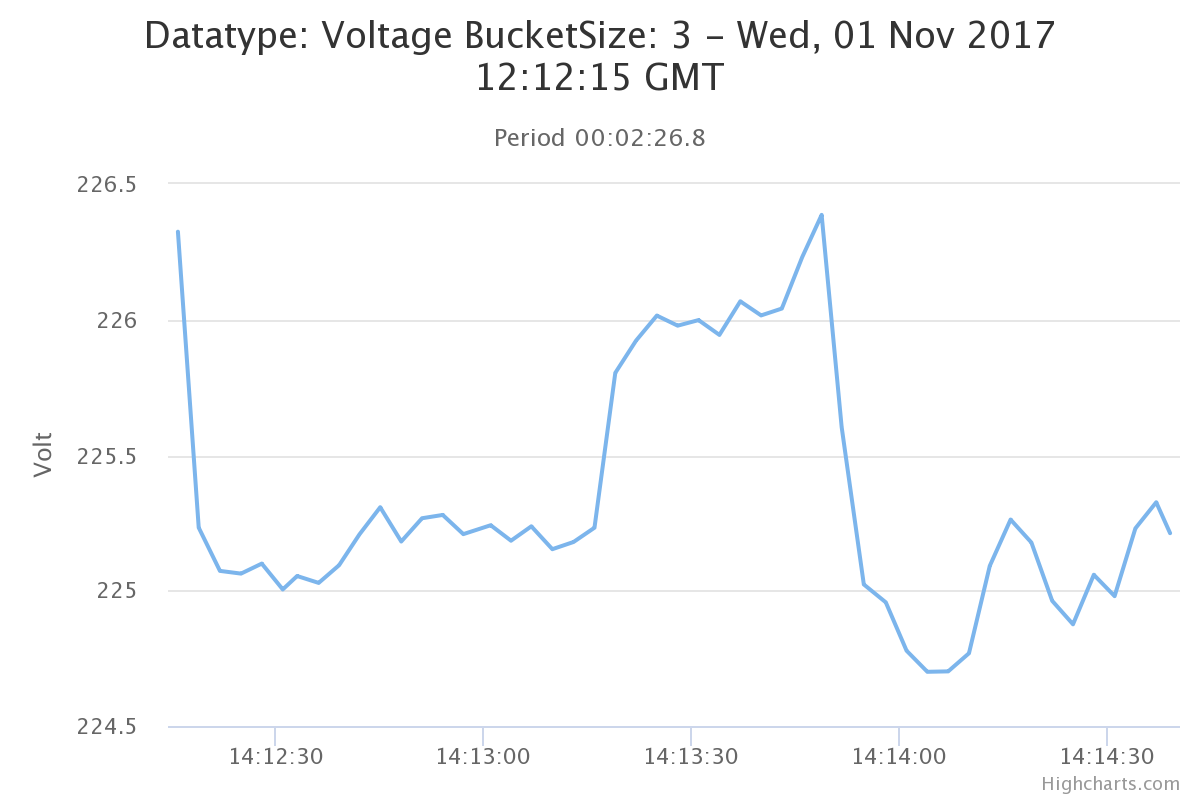
\includegraphics[width=0.8\textwidth]{SpannungsverlaufSenseo1}
        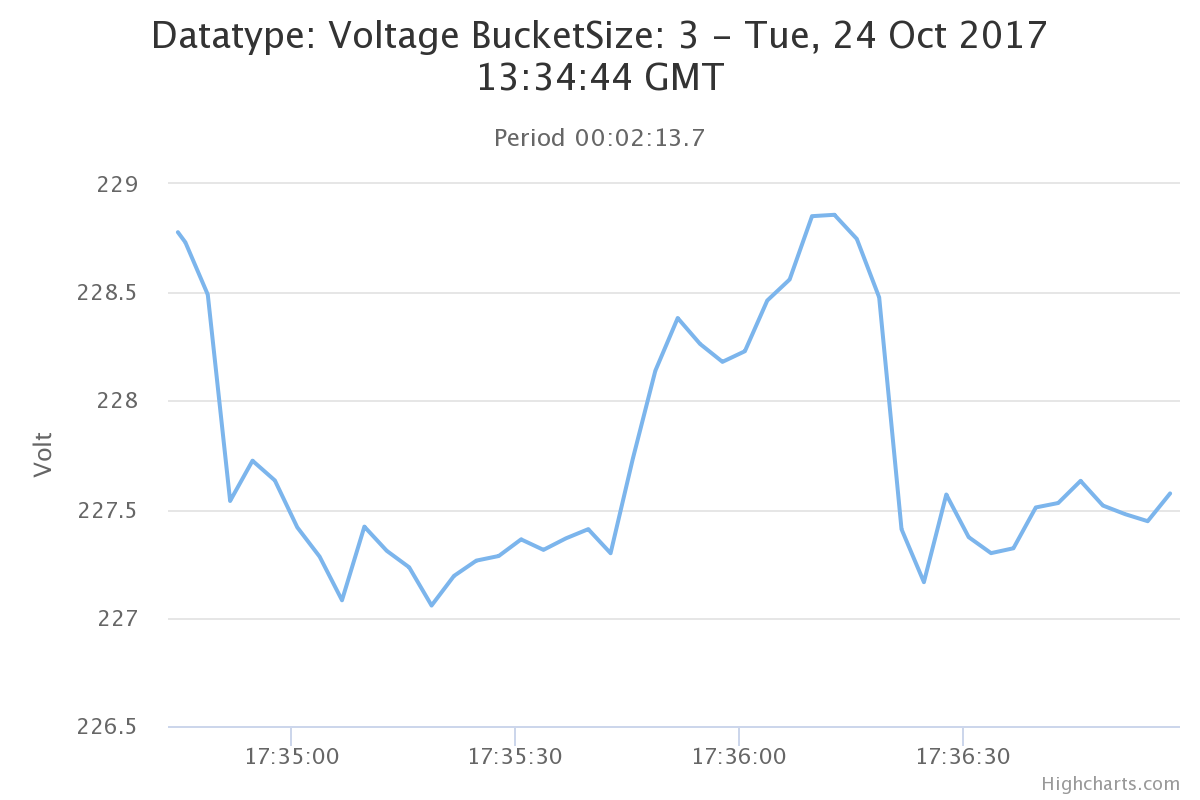
\includegraphics[width=0.8\textwidth]{SpannungsverlaufSenseo2}
        \caption{Spannungsverlauf der Senseo Kaffeemaschine mit einer Klasse von je 3 Datenpunkten zu 2 verschiedenen Zeitpunkten}
        \label{fig:SpannungsverlaufSenseo}
    \end{figure}

    \noindent
    Bei der manuellen Analyse der Mikrowelle können bei Analyse des Spannungs- oder Frequenzverlaufs leider keine hervorstechenden Merkmale oder Gemeinsamkeiten erkannt werden.
    Somit wird die Mikrowelle demnach einen anderen Einfluss auf doe Netzaktivität ausüben.
    Wie bei dem Vergleich der verschiedenen harmonischen Oberwellen zu sehen ist (siehe Schaubild \ref{fig:3OberwelleMikrowelle}), besteht eine große Ähnlichkeit der Kurven der dritten harmonischen Welle.\\
    \newline

    \begin{figure}[h]
        \centering
        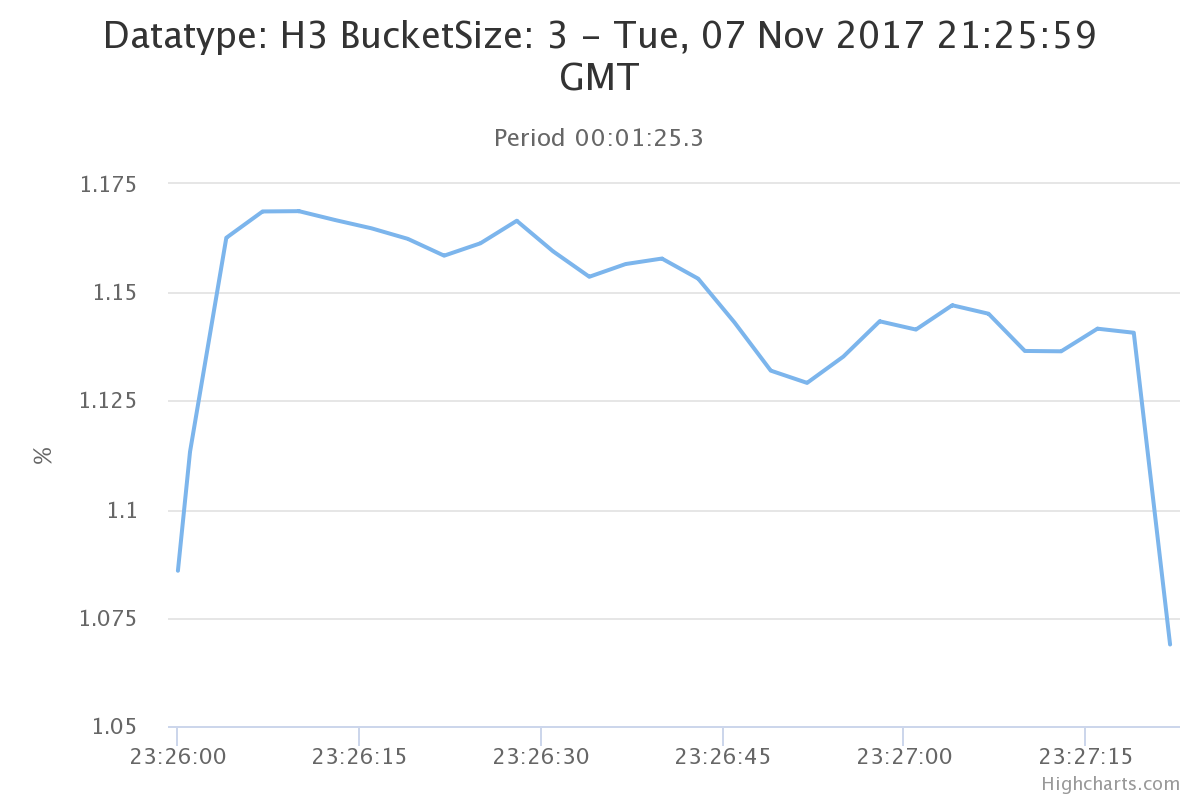
\includegraphics[width=0.8\textwidth]{3OberwelleMikrowelle1}
        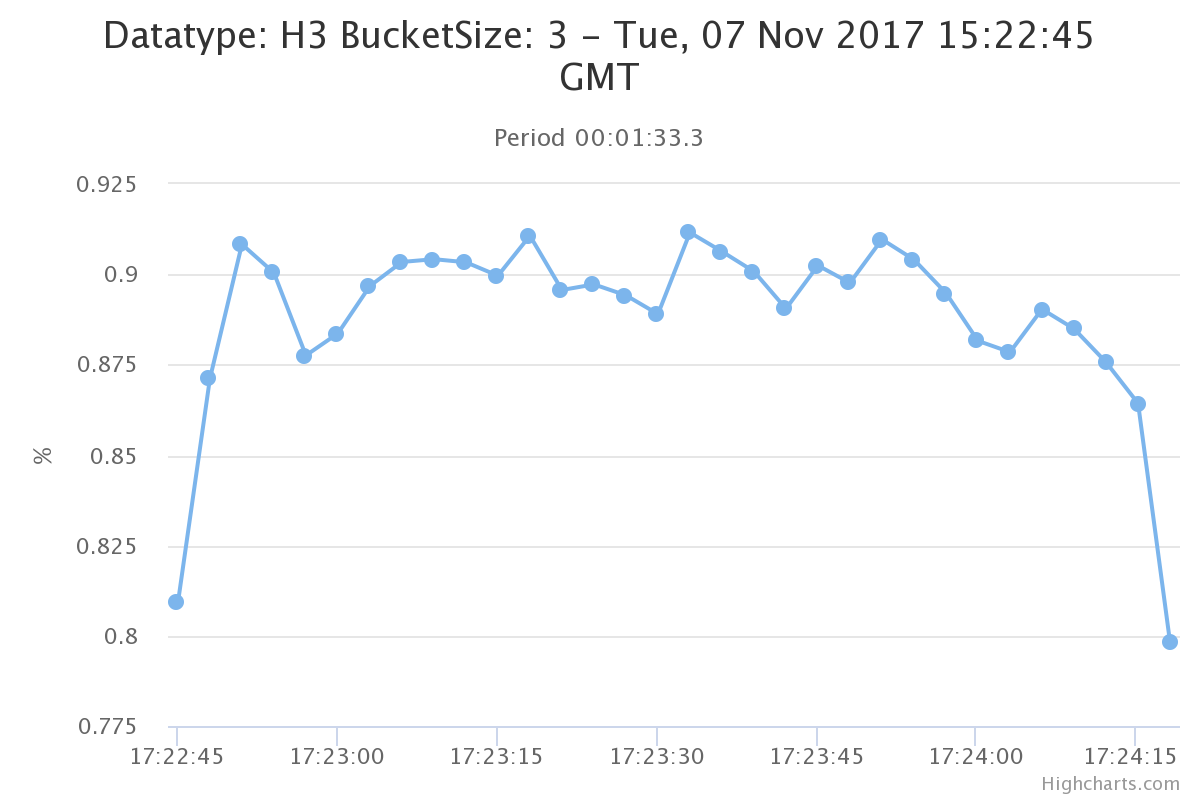
\includegraphics[width=0.8\textwidth]{3OberwelleMikrowelle2}
        \caption{Verlauf der 3. harmonischen Oberwelle einer Mikrowelle mit einer Klasse von je 3 Datenpunkten zu 2 verschiedenen Zeitpunkten}
        \label{fig:3OberwelleMikrowelle}
    \end{figure}

    \noindent
    Wie dieser Abschnitt zeigt können schon mit bloßen Auge bestimmte Auswirkungen der verschiedenen Geräte erkannt werden.
    Auch wenn manchmal einige Störungen auftreten und den Verlauf verfälschen sollte es demnach möglich sein diese Geräte herauszufiltern.
    Da nun das manuelle Durchsuchen von langen Zeitspannen sehr mühselig ist wird nun weiterführend beschrieben diese Klassifizierung der Geräte auf maschinellem Lernen abzubilden.

\section{Vorbereiten der Daten}

\section{Neuronales Netz}

\section{Trainingsprozess}

\section{Auswertung der Ergebnisse}
